\documentclass[a4paper, 11pt]{article}

\usepackage[french]{babel}
\usepackage[french, noheader]{packages/sleek}
\usepackage[nomessages]{fp}
\usepackage{packages/sleek-title}
\usepackage{tabularx}

\addbibresource{references.bib}
\setcounter{tocdepth}{1}
\setlength{\emergencystretch}{3em}

\newcolumntype{Y}{>{\raggedright\arraybackslash}X}
\newcommand{\ahat}{\hat\alpha}
\newcommand{\phat}{\hat p}
\newcommand{\Q}[1]{\textbf{Q#1}}

\title{Où naît le flou ?}
\subtitle{Régression, diffusion et jetons discrets face à un futur incertain, \\ mesurés sur un jeu dont le hasard est connu}
\author{Cédric \textsc{Dada}}
\date{24 novembre 2026}

\begin{document}

\maketitle

\section*{Résumé}

Un modèle du monde prédit l'image suivante d'un environnement à partir des images passées et de l'action jouée. Quand le
futur est incertain, la façon dont ce modèle est entraîné décide de ce qu'il dessine : une régression à l'erreur
quadratique tend vers la moyenne des futurs possibles, donc vers une image floue, alors qu'un modèle génératif est censé
en tirer un seul. Sur des jeux réels, cette différence se constate mais se mesure mal, faute de connaître la vraie loi des
futurs. Nous avons construit un mini-jeu de $64\times64$ pixels dont le seul hasard est une bifurcation : un ennemi part à
droite avec une probabilité $p$ réglable, à gauche sinon. Les deux images possibles se calculent exactement, ce qui permet
de classer chaque prédiction comme nette (l'une ou l'autre branche), floue (un mélange des deux) ou incorrecte. Nous y
comparons trois familles de prédicteurs à budget d'entraînement égal : une régression (U-Net, erreur quadratique), un modèle
de diffusion (EDM) échantillonné en 1 à 20 pas, et un modèle à jetons discrets (VQ-VAE suivi d'un Transformer), soit
25 entraînements et 46,6~heures de GPU. La régression produit le mélange attendu dans 97,6~\% des cas, avec une erreur à
1,01 fois le minimum théorique. La diffusion à 3 pas tranche nettement dans 90,7~\% des cas et respecte en moyenne la
probabilité des branches ($\phat = 0{,}313$ pour $p = 0{,}3$), mais un seul pas d'échantillonnage ne produit pas l'image
moyenne : il donne des images bruitées hors des deux futurs, ce qu'un balayage du niveau de bruit initial relie au peu
d'exemples vus à fort bruit pendant l'entraînement. Les jetons tranchent eux aussi, mais déplacent souvent l'agent d'un ou
deux pixels ; augmenter la taille du dictionnaire réduit ces erreurs. Enfin, le flou n'est pas toujours un défaut : lu par un
détecteur de contact affine en l'image, le mélange de la régression estime le risque de collision à un pas mieux que les
modèles qui tranchent (erreur 0,03 contre 0,16), mais cet avantage disparaît dès que le modèle doit enchaîner ses propres
prédictions.

\vspace{1em}
\tableofcontents
\newpage

%% ============================================================================================================
\section{Introduction}\label{sec:intro}

Un modèle du monde, au sens de \textcite{ha2018worldmodels}, est un réseau qui apprend la dynamique d'un environnement
pour qu'un agent puisse s'y entraîner ou y planifier sans interagir avec le monde réel. Dans les travaux récents sur les
jeux vidéo, sa composante centrale prédit l'image suivante à partir de quelques images passées et de l'action jouée :
DIAMOND le fait par diffusion directement dans l'espace des pixels \parencite{alonso2024diamond}, IRIS en compressant
chaque image en jetons discrets prédits par un Transformer \parencite{micheli2023iris}.

Ces prédicteurs se heurtent tous à la même difficulté quand le futur n'est pas déterminé par le passé. Si un adversaire
peut aller à gauche ou à droite, il existe deux images suivantes plausibles. Un réseau entraîné à minimiser l'erreur
quadratique converge vers leur moyenne pondérée, une image où l'adversaire apparaît à moitié aux deux endroits. Ce flou
a été observé en prédiction vidéo \parencite{mathieu2016deep, babaeizadeh2018sv2p}, et il a une justification théorique
précise : l'estimateur d'erreur quadratique minimale moyenne les explications possibles, tandis qu'un échantillonnage
parfait de la loi a posteriori produit une image nette, au prix d'une erreur quadratique deux fois plus grande
\parencite{blau2018perception}. DIAMOND rapporte le même phénomène sur le jeu \emph{Boxing} : un seul pas de débruitage
produit une image floue qui moyenne les mouvements possibles du joueur adverse, alors que plusieurs pas s'engagent sur
l'un d'eux \parencite[§5.2]{alonso2024diamond}.

Ces constats restent qualitatifs. Sur un jeu réel, on ignore la loi exacte des futurs : on peut voir qu'une image est
floue, mais pas dire si elle est le bon mélange, ni si un modèle qui tranche choisit chaque branche aussi souvent qu'il le
devrait. Ce travail part de cette lacune. Nous avons construit un environnement minimal où tout est connu : un seul
événement aléatoire, de probabilité $p$ réglable, dont les deux issues se rendent exactement. Chaque prédiction peut alors
être située par rapport aux deux futurs possibles, et l'erreur de chaque modèle comparée à un minimum théorique calculable.

Sur ce banc d'essai, nous comparons trois familles de prédicteurs entraînées dans les mêmes conditions, et nous
répondons à cinq questions de recherche, issues chacune d'un constat ou d'une question ouverte de la littérature
(section~\ref{sec:questions}). Nos principaux résultats sont les suivants.

\begin{itemize}
  \item La régression produit le mélange théorique avec une grande exactitude : son erreur vaut 1,01 fois le minimum de
  Bayes, et la position de ses images entre les deux futurs suit $p$.
  \item La diffusion tranche dès 3 pas et respecte en moyenne la probabilité des branches, avec une dispersion d'une
  graine d'entraînement à l'autre de l'ordre de $\pm 0{,}05$. À un seul pas, elle ne produit pas la moyenne mais des images
  hors des deux futurs ; un diagnostic supplémentaire relie cet échec aux niveaux de bruit rarement vus à l'entraînement.
  \item Les jetons discrets tranchent aussi, mais commettent des erreurs de position sur le reste de l'image, qui diminuent
  quand le dictionnaire grandit. La conservation d'un petit objet de $2\times2$ pixels, elle, ne départage pas les
  modèles : elle est proche de 98~\% pour tous.
  \item Pour estimer un risque de collision à un pas, l'image floue de la régression est la meilleure des trois, à
  condition de la lire avec un détecteur affine. L'avantage s'inverse dès que la prédiction s'enchaîne sur plusieurs pas.
\end{itemize}

%% ============================================================================================================
\section{Questions de recherche et travaux qui les motivent}\label{sec:questions}

Avant de lancer les entraînements, nous avons fixé pour chaque question ce que nous nous attendions à observer et le
critère qui permettrait de trancher. Ces critères sont rassemblés en annexe~\ref{app:criteres} ; ils ont été écrits avant
toute mesure sur un modèle entraîné, pour qu'un résultat décevant ne puisse pas être réinterprété après coup. Une
réponse peut être positive, négative, ou non tranchée quand les données ne permettent ni l'un ni l'autre.

\paragraph{\Q1. Une régression produit-elle bien le mélange des futurs, et les modèles génératifs tranchent-ils ?}
Le flou des modèles entraînés à l'erreur quadratique est connu depuis les premiers travaux de prédiction vidéo
\parencite{mathieu2016deep}, et SV2P l'a illustré sur un jeu jouet à direction aléatoire, où le modèle déterministe
prédit la moyenne \parencite{babaeizadeh2018sv2p}. La théorie dit même précisément quelle image attendre
\parencite{blau2018perception}. Ce qu'aucun de ces travaux ne mesure, faute de vérité terrain, c'est l'écart entre l'image
prédite et le mélange exact. Notre question est donc quantitative : la régression atteint-elle le minimum théorique, et
les deux familles génératives produisent-elles des images nettes dans la grande majorité des cas ?

\paragraph{\Q2. Le nombre de pas d'échantillonnage de la diffusion change-t-il ce comportement ?}
L'observation de DIAMOND sur \emph{Boxing} suggère qu'un modèle de diffusion échantillonné en un seul pas se comporte
comme une régression \parencite[§5.2]{alonso2024diamond}. La formulation EDM, sur laquelle repose DIAMOND, ne traite pas
ce régime : sa figure consacrée au nombre d'évaluations commence à 7 \parencite{karras2022edm}. Nous avons voulu mesurer, sur les mêmes réseaux, la part d'images floues à 1, 3, 5 et 20 pas.

\paragraph{\Q3. Les images nettes respectent-elles la probabilité des branches ?}
Un modèle qui tranche peut le faire avec un biais. \textcite[§3.2.2]{song2019generative} montrent qu'une dynamique de
Langevin retrouve mal le poids relatif de deux modes, même avec le score exact ; \textcite{um2024minority} décrivent un
biais des débruiteurs appris vers les échantillons majoritaires. Des travaux récents commencent à évaluer la calibration
des générateurs vidéo contre des lois connues \parencite{sadeghi2026calibench} ou sur des jeux synthétiques aux futurs
énumérables \parencite{porcher2026flowwm}. Notre jeu s'y prête directement : la part de la branche A parmi les images
nettes, notée $\phat$, doit valoir $p$.

\paragraph{\Q4. La taille du dictionnaire des jetons affecte-t-elle les petits détails ?}
Un modèle à jetons représente chaque image par un nombre fini de codes appris \parencite{vandenoord2017vqvae}. Le titre
même de DIAMOND, \enquote{les détails visuels comptent}, met en avant ce que cette compression peut perdre
\parencite{alonso2024diamond}. Notre raisonnement, qui ne vient pas d'un article, était le suivant : un objet de
$2\times2$ pixels, un quart d'une case de la grille de jetons, n'a peut-être pas de code propre quand le dictionnaire est
petit. Nous avons fait varier sa taille $K$ de 64 à 1\,024 codes.

\paragraph{\Q5. Le flou change-t-il une décision ?}
Mesurer la netteté ne dit pas si elle compte pour l'usage d'un modèle du monde. PETS planifie en propageant soit
l'espérance de la prédiction, soit des tirages, et avertit que de petits biais du modèle s'accumulent vite le long d'une
trajectoire \parencite[§5.2]{chua2018pets}. \textcite[§4.1]{lambert2020objective} mesurent une corrélation de $-0{,}06$ à
$0{,}59$ entre la précision d'un modèle et la qualité du contrôle obtenu, sur plus de 1\,000 modèles. Nous avons mesuré l'effet du flou sur une décision simple, l'estimation du risque de toucher l'ennemi dans les $k$ prochains pas, avec
deux façons de lire l'image. Notre propre raisonnement prévoyait un résultat contrasté : un lecteur affine appliqué au
mélange exact $pA + (1-p)B$ renvoie exactement le bon risque, le flou ne devrait donc gêner qu'un lecteur à seuil.

%% ============================================================================================================
\section{Dispositif expérimental}\label{sec:dispositif}

\subsection{Un jeu dont le hasard tient en une seule bifurcation}

Le jeu se joue sur une image RGB de $64\times64$ pixels (figure~\ref{fig:jeu}). L'agent, un carré bleu de $4\times4$
pixels, se déplace de 2 pixels par pas selon l'une des cinq actions (immobile, haut, bas, gauche, droite). Il doit ramasser
un petit objet jaune de $2\times2$ pixels (+1 point) en évitant un ennemi rouge ($-1$ point par contact). Quatre piliers et un
mur d'enceinte l'arrêtent. Un obstacle mobile gris clair rebondit sur les murs de façon entièrement déterministe : il sert
de témoin, puisqu'un modèle n'a aucune raison de le prédire flou.

L'ennemi va et vient sur un rail horizontal au centre de l'image, à 6 pixels par pas. Chaque fois qu'il repasse au centre,
soit un pas sur six, il choisit sa direction au hasard : droite avec la probabilité $p$, gauche sinon. C'est la
\emph{bifurcation}, et c'est la seule source de hasard du jeu. Les deux positions possibles au pas suivant sont distantes de
12 pixels, si bien que les deux images futures, notées $A$ (droite) et $B$ (gauche), ne diffèrent que par la position de
l'ennemi. Comme le rendu est une fonction exacte de l'état du jeu, on peut calculer $A$ et $B$ pour n'importe quel état :
c'est le \emph{rendu contrefactuel} sur lequel repose toute la mesure.

\begin{figure}[ht]
  \centering
  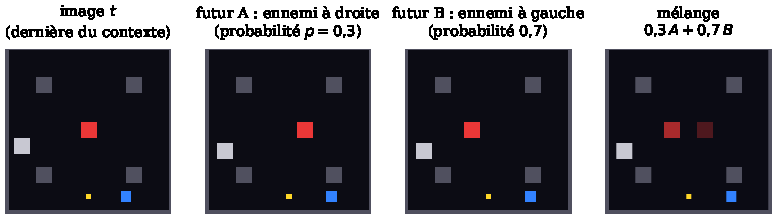
\includegraphics[width=\linewidth]{figures/fig_jeu.pdf}
  \caption{Un état de bifurcation et ses deux futurs. L'ennemi (rouge) est au centre de son rail : au pas suivant, il
  sera à droite avec une probabilité $p = 0{,}3$ (futur A) ou à gauche (futur B). L'image de droite est la moyenne
  pondérée des deux futurs, que devrait produire un modèle entraîné à l'erreur quadratique. L'agent est le carré bleu,
  le petit objet le carré jaune, l'obstacle mobile le carré gris clair.}
  \label{fig:jeu}
\end{figure}

\subsection{Données}

Les épisodes durent 100 pas et sont joués par deux bots : un bot aléatoire et un bot glouton qui se dirige vers le petit
objet. Chaque jeu de données d'entraînement compte 400\,000 transitions par valeur de $p$, avec un jeu de validation
séparé de 20\,000 transitions. Le modèle reçoit les 4 dernières images et l'action, et doit prédire l'image suivante. Le
jeu de test contient 2\,000 états de bifurcation figés, communs à tous les modèles. Train, validation et test sont tirés
de flux aléatoires distincts, et un test automatique vérifie qu'aucun contexte de test n'apparaît à l'entraînement.

La taille du jeu d'entraînement a été fixée après un premier essai. Avec 100\,000 transitions, une régression voyait
chaque transition 22 fois et finissait par mémoriser l'issue des bifurcations vues : sa perte d'entraînement descendait à
0,46 fois le minimum théorique, ce qui est impossible sans connaître la branche tirée, et sa perte de validation remontait
de 49~\%. Avec 400\,000 transitions (5,6 passages), ce phénomène disparaît. L'annexe~\ref{app:surapprentissage} détaille
cet essai, écarté de toutes les analyses.

\subsection{Trois familles de prédicteurs}

Les trois familles ont des tailles proches, de 5,9 à 6,6 millions de paramètres (tableau~\ref{tab:familles}), et voient le même nombre d'images : 34\,800 pas d'optimisation par lots de 64, soit 2\,227\,200 exemples. Aucune moyenne
glissante des poids n'est utilisée, pour qu'aucune famille ne bénéficie d'un réglage propre. Les détails d'entraînement
sont en annexe~\ref{app:details}.

\begin{table}[ht]
  \centering\small
  \begin{tabularx}{\linewidth}{@{}l>{\raggedright\arraybackslash}p{4.3cm}Yr@{}}
    \toprule
    Famille & Modèle & Ce que la sortie représente & Paramètres \\
    \midrule
    Régression & U-Net \parencite{ronneberger2015unet}, une passe, erreur quadratique & l'espérance conditionnelle de l'image suivante & 5,87~M \\
    Diffusion & même U-Net, préconditionnement et bruit d'EDM \parencite{karras2022edm}, échantillonneur d'Euler à $n$ pas & un tirage de la loi de l'image suivante & 6,01~M \\
    Jetons & VQ-VAE \parencite{vandenoord2017vqvae} sur une grille de $8\times8$ jetons, puis Transformer causal \parencite{vaswani2017attention}, température 1 & un tirage, jeton par jeton, parmi $K$ codes & 5,91 à 6,59~M \\
    \bottomrule
  \end{tabularx}
  \caption{Les trois familles comparées. Le modèle à jetons répartit son budget entre le VQ-VAE (40~\% des pas) et le
  Transformer (60~\%). Sa taille varie avec le dictionnaire : 5,91~M de paramètres à $K = 64$, 6,04~M à $K = 256$,
  6,59~M à $K = 1\,024$.}
  \label{tab:familles}
\end{table}

\subsection{Mesurer le flou sans juger à l'œil}\label{sec:instrument}

\paragraph{Position entre les deux futurs.} Pour chaque état de test, on connaît les deux images possibles $A$ et $B$.
Une prédiction $\hat y$ est projetée sur le segment qui les relie, comme on projette une couleur sur le segment
premier plan–fond en détourage d'images \parencite{wang2007matting} :
\begin{equation}
  \ahat = \operatorname{clip}_{[0,1]}\!\left(\frac{\langle \hat y - B,\, A - B\rangle}{\delta^2}\right),
  \qquad
  \rho = \frac{\lVert \hat y - (\ahat A + (1-\ahat) B)\rVert}{\delta},
  \qquad \delta = \lVert A - B\rVert .
\end{equation}
La coordonnée $\ahat$ dit où l'image se situe entre $B$ ($\ahat = 0$) et $A$ ($\ahat = 1$) ; $\rho$ dit à quelle distance du
segment elle se trouve. Avec un seuil $\varepsilon = 0{,}2$, une prédiction est classée \emph{nette-A} si
$\ahat \ge 0{,}8$, \emph{nette-B} si $\ahat \le 0{,}2$, \emph{floue} entre les deux, et \emph{autre} si $\rho$ dépasse un
seuil $\rho_{\max}$, c'est-à-dire si l'image n'est ni l'un des futurs ni leur mélange (objet déplacé ou disparu, bruit).

\paragraph{Calibrer le seuil sans regarder les modèles.} Le seuil $\rho_{\max}$ est réglé une fois pour toutes sur des
images synthétiques : des futurs exacts auxquels on ajoute un bruit gaussien d'écart-type 0,01, dont on retient le quantile
à 99,5~\% de $\rho$. Sur les 8\,000 paires des quatre jeux de test, on obtient $\rho_{\max} = 0{,}160$. Avec ce seuil, le
classifieur retrouve la position des mélanges synthétiques avec une erreur moyenne de 0,001 sur $\ahat$ et classe
correctement 99,5~\% des images pures bruitées. La part d'images \enquote{autre} dépend de ce choix et ne doit pas être lue
comme une mesure absolue : à un seuil deux fois plus bas, plus aucune image pure bruitée n'est reconnue. Recalculées sur
les sorties des modèles, les parts d'images floues et \enquote{autre} varient pourtant peu entre la moitié et le double du seuil
retenu (annexe~\ref{app:sensibilite}).

\paragraph{Un minimum théorique pour l'erreur quadratique.} Pour un état de bifurcation, un prédicteur qui ignore la
branche tirée commet une erreur quadratique moyenne au moins égale à
\begin{equation}
  \min_{\hat y}\; \mathbb E\,\lVert \hat y - Y\rVert^2 = p\,(1-p)\,\delta^2 ,
  \qquad\text{atteint pour } \hat y^\star = p\,A + (1-p)\,B ,
\end{equation}
puisque $\mathbb E\lVert\hat y - Y\rVert^2 = p\lVert \hat y - A\rVert^2 + (1-p)\lVert \hat y - B\rVert^2$. C'est le
plancher de Bayes. Un générateur parfait, qui tire $A$ ou $B$ indépendamment de la vraie issue, se trompe de branche avec la
probabilité $2p(1-p)$ et a donc une erreur double. Nous rapportons le rapport entre l'erreur d'un modèle et ce plancher : il
vaut 1 pour une régression idéale et 2 pour un générateur idéal. Ce rapport est calculé contre la loi exacte des deux
futurs ; calculé contre l'issue effectivement tirée, il permet aussi de détecter un modèle qui \enquote{connaîtrait} la
branche, son rapport tombant alors sous 1.

\paragraph{Une variante restreinte au rail de l'ennemi.} Comme $\rho$ est normalisé par $\delta$, qui ne mesure que le
déplacement de l'ennemi, un agent décalé d'un seul pixel suffit à classer une image comme \enquote{autre}, même si la
bifurcation est parfaitement tranchée. Après la première série de résultats, nous avons ajouté une mesure secondaire, déclarée
exploratoire avant toute analyse : les mêmes $\ahat$ et $\rho$ calculés sur les seuls pixels où $A$ et $B$ diffèrent,
dilatés de 2 pixels. Elle sépare deux questions, \enquote{la bifurcation est-elle tranchée ?} et \enquote{le reste de l'image
est-il juste ?}. Elle réutilise le seuil $\rho_{\max}$ calibré sur l'image entière ; or, sur le rail, le même bruit
synthétique donne un quantile de 0,036 seulement. Ses \enquote{autre} sont donc un minorant.

\paragraph{Autres mesures.} Le \emph{rappel du petit objet} est la part des prédictions où l'objet de $2\times2$ pixels
est retrouvé à sa place. Le \emph{suivi à 16 pas} est obtenu en laissant chaque modèle enchaîner 16 prédictions sur
250 états de test, en lui redonnant à chaque pas ses propres images : c'est la part des trajectoires où l'agent et l'obstacle
mobile sont encore retrouvés à moins de 3 pixels de leur vraie position au 16\textsuperscript{e} pas.

\subsection{Contrôles}

Trois modèles supplémentaires vérifient que l'instrument mesure bien ce qu'on lui prête. Un \emph{régresseur oracle}
reçoit en entrée la branche réellement tirée : il n'a plus de raison de produire du flou. Une régression et une diffusion
sont entraînées à $p = 0$, où le jeu devient déterministe : on ne devrait y voir aucun flou, quel que soit le nombre de pas.
Pour chaque contrôle, le critère était de moins de 5~\% d'images floues.

\subsection{Plan d'expériences et statistiques}

Le c\oe ur de l'étude compare les trois familles à $p = 0{,}3$ sur trois graines d'entraînement chacune. S'y ajoutent les
trois contrôles, un axe $K$ (jetons à $K = 64$ et $K = 1\,024$, trois graines chacun), une grille de $16\times16$ jetons à
$K = 256$ (une graine) et un axe $p$ ($p = 0{,}1$ et $0{,}5$ pour les trois familles, une graine). Les 25 entraînements ont
demandé 46,6~heures sur un GPU NVIDIA T4 : 2,3 à 2,7~heures pour une régression ou une diffusion, environ 1~heure pour un
modèle à jetons, 3,2~heures pour la grille fine.

Avec trois graines, les écarts entre familles sont jugés à l'aide de seuils exprimés en écarts-types, issus de la loi de
Student et corrigés par Bonferroni pour les trois comparaisons principales menées simultanément : un écart doit dépasser
3,23 écarts-types poolés pour une comparaison entre modèles différents, et 4,42 écarts-types des différences pour une
comparaison appariée (les mêmes réseaux échantillonnés de deux façons). Ces règles sont des garde-fous pour très peu de
graines, pas des tests de significativité au sens habituel : un écart sous le seuil n'est pas une absence d'effet.

%% ============================================================================================================
\section{Résultats}\label{sec:resultats}

\subsection{L'instrument et les contrôles se comportent comme prévu}

Avant toute mesure sur un modèle, le classifieur passe le contrôle sur images synthétiques décrit plus haut. Les trois
régressions du c\oe ur ont un rapport au plancher de Bayes de 1,011, 1,016 et 1,013, dans l'intervalle $[1{,}00 ; 1{,}10]$
fixé à l'avance, et leur rapport calculé contre l'issue tirée (0,986 à 0,995) ne trahit aucune fuite d'information sur la
branche. L'oracle produit 98,8~\% d'images nettes et aucune image floue. À $p = 0$, ni la régression ni la diffusion à un pas
ne produisent d'image floue. Ce dernier contrôle aura une importance particulière pour la question~2 : la diffusion à un pas
y donne bien zéro image floue, mais 100~\% d'images \enquote{autre}, alors même que le jeu est déterministe.

\subsection{Q1 : la régression produit le mélange exact, les modèles génératifs tranchent}

La figure~\ref{fig:echantillons} montre trois états de test tels que les voit chaque famille, et le
tableau~\ref{tab:principal} rassemble les mesures. La réponse à la première question est positive, et nettement. Sur les
2\,000 états de test, la régression produit une image floue dans 97,6~\% des cas en moyenne sur trois graines
(96,7 à 98,2~\%). Son erreur vaut 1,01 fois le plancher de Bayes et sa coordonnée moyenne $\ahat$ vaut 0,297 pour $p = 0{,}3$ :
elle n'est pas \enquote{à peu près floue}, elle dessine le mélange théorique. La diffusion à 3 pas produit 90,7~\% d'images
nettes (89,1 à 91,6~\%) et 4,5~\% d'images floues, au-dessus des 90~\% et sous les 10~\% fixés à l'avance. Son erreur vaut
2,02 fois le plancher, la valeur attendue d'un générateur qui tire une branche au hasard.

\begin{figure}[ht]
  \centering
  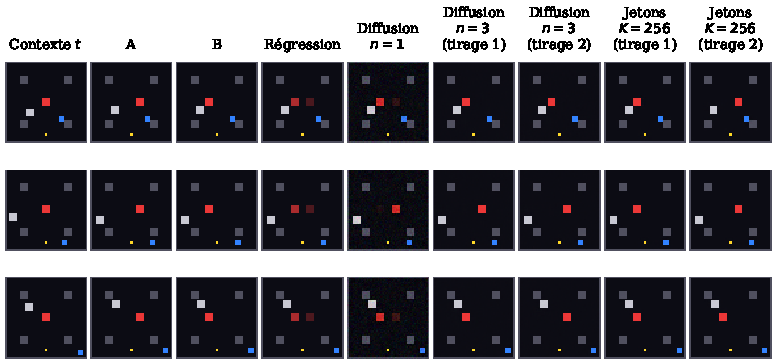
\includegraphics[width=\linewidth]{figures/fig_echantillons.pdf}
  \caption{Trois états de test du jeu de test (lignes), avec les deux futurs possibles A et B, puis la prédiction de chaque
  famille (graine 0, $p = 0{,}3$). La régression dessine l'ennemi aux deux positions, plus pâle à droite (poids 0,3) qu'à
  gauche. La diffusion à un pas produit le même mélange mais sur un fond granuleux. À 3 pas, la diffusion et les jetons
  dessinent un ennemi net, à droite ou à gauche selon le tirage.}
  \label{fig:echantillons}
\end{figure}

\begin{table}[ht]
  \centering\footnotesize\setlength{\tabcolsep}{4pt}
  \begin{tabular}{@{}lrrrrrrrr@{}}
\toprule
& \multicolumn{3}{c}{image entière (\%)} & rail & MSE / & & rappel & suivi \\
\cmidrule(lr){2-4}
Modèle & floue & nette & autre & autre (\%) & plancher & $\hat p$ & (\%) & 16 pas (\%) \\
\midrule
Régression & 97,6 & 1,0 & 1,4 & 0,1 & 1,01 & -- & 98,8 & 100 \\
Diffusion, $n=1$ & 0,0 & 0,0 & 100,0 & 4,5 & 2,12 & -- & 98,6 & 76 \\
Diffusion, $n=3$ & 4,5 & 90,7 & 4,8 & 1,2 & 2,02 & 0,313 & 98,8 & 81 \\
Diffusion, $n=5$ & 0,3 & 95,4 & 4,3 & 1,2 & 1,97 & 0,265 & 98,8 & 84 \\
Diffusion, $n=20$ & 0,0 & 96,5 & 3,5 & 0,6 & 2,06 & 0,302 & 98,8 & 86 \\
Jetons, $K=64$ & 0,0 & 36,7 & 63,3 & 17,2 & 3,51 & 0,280 & 98,1 & 4 \\
Jetons, $K=256$ & 0,0 & 46,8 & 53,2 & 15,6 & 3,46 & 0,277 & 98,2 & 7 \\
Jetons, $K=1\,024$ & 0,0 & 67,5 & 32,5 & 10,8 & 2,84 & 0,287 & 98,4 & 21 \\
Jetons, $K=256$, grille $16\times16$ $^\dagger$ & 0,0 & 60,8 & 39,2 & 13,6 & 3,15 & 0,291 & 98,2 & 13 \\
Régresseur oracle $^\dagger$ & 0,0 & 98,8 & 1,2 & 0,0 & 1,98 & 0,287 & 98,8 & -- \\
\bottomrule
\end{tabular}

  \caption{Mesures principales à $p = 0{,}3$ sur les 2\,000 états de test, moyennées sur trois graines
  ($^\dagger$ : une seule graine). \emph{Rail} : part d'images \enquote{autre} quand la mesure est restreinte aux pixels du rail
  de l'ennemi. $\phat$ : part de la branche A parmi les images nettes ; il n'est pas donné pour la régression, qui ne produit
  que 8 à 39 images nettes par graine. Le suivi à 16 pas n'est pas mesuré pour l'oracle, qui a besoin de la branche tirée à
  chaque pas.}
  \label{tab:principal}
\end{table}

Les modèles à jetons tranchent eux aussi : ils ne produisent aucune image floue. Mais une part importante de leurs
prédictions, 53~\% à $K = 256$, est classée \enquote{autre}. La mesure restreinte au rail de l'ennemi
(figure~\ref{fig:classes}) explique ce chiffre : sur le rail, cette part tombe à 16~\%. La plupart de ces images ont tranché la bifurcation correctement, mais commettent une erreur ailleurs. L'examen de 25 d'entre elles montre surtout un
agent décalé d'un ou deux pixels, ou dédoublé à la frontière entre deux jetons : 58~\% de l'écart au segment $[B, A]$ se
concentre sur les pixels de l'agent. Le même découpage confirme la lecture de la régression : ses rares images
\enquote{autre} (1,4~\%) deviennent floues quand on regarde le seul rail, leur écart venant du reste de l'image.

\begin{figure}[ht]
  \centering
  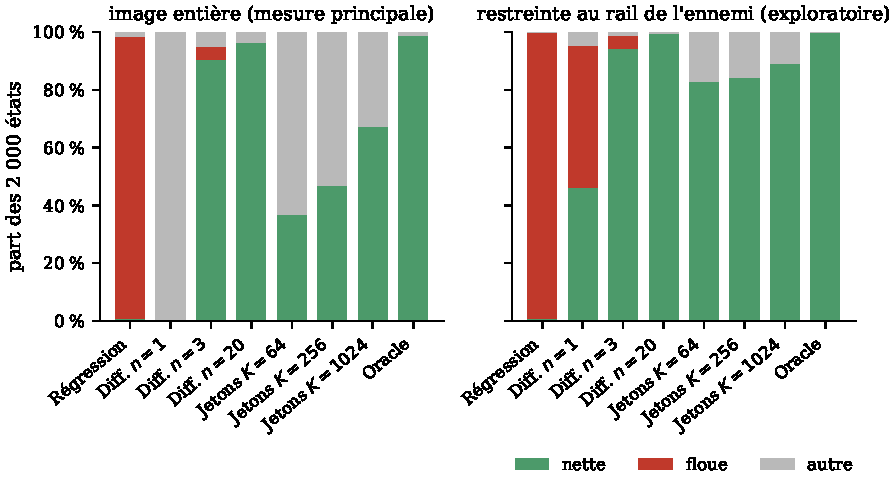
\includegraphics[width=\linewidth]{figures/fig_classes.pdf}
  \caption{Répartition des 2\,000 prédictions de test entre images nettes, floues et \enquote{autre}, moyenne sur trois graines
  (une pour l'oracle). À gauche, la mesure principale sur l'image entière ; à droite, la variante exploratoire restreinte au
  rail de l'ennemi, qui ignore les erreurs commises ailleurs dans l'image.}
  \label{fig:classes}
\end{figure}

\subsection{Q2 : un seul pas de diffusion ne produit pas la moyenne}

La deuxième question reçoit une réponse négative, mais pas pour la raison attendue. Nous nous attendions, comme sur
\emph{Boxing}, à ce qu'un seul pas d'échantillonnage produise des images floues, et à un écart d'au moins 10 points avec le
cas à 3 pas. Or la diffusion à un pas ne produit \emph{aucune} image floue sur les trois graines : toutes ses prédictions sont
classées \enquote{autre}, et son erreur vaut 2,12 fois le plancher. La figure~\ref{fig:echantillons} montre pourquoi : l'image
contient bien un mélange des deux positions de l'ennemi, mais posé sur un fond granuleux qui l'éloigne du segment $[B, A]$.
Le contrôle à $p = 0$ produit le même résultat sur un jeu sans aucun hasard, ce qui montre que cet échec n'est pas lié à la
bifurcation. Restreinte au rail de l'ennemi, la mesure donne une image floue dans 46 à 53~\% des cas et nette dans 44 à
50~\%, selon la graine.

\paragraph{Diagnostic : le niveau de bruit de départ.} Un échantillonneur d'Euler à un pas part d'un bruit pur de niveau
$\sigma_{\max} = 80$ et renvoie directement la sortie du débruiteur. En théorie, cette sortie est la moyenne conditionnelle.
Mais pendant l'entraînement, le niveau de bruit suit la loi log-normale d'EDM, $\ln\sigma \sim \mathcal N(-1{,}2\,;\,1{,}2^2)$
\parencite{karras2022edm} : sur 2\,227\,200 exemples, seuls 4 avaient un bruit supérieur à 80, et 525 un bruit supérieur
à 20, contre 21\,400 au-dessus de 5. Le réseau n'a presque jamais appris à débruiter au niveau où l'échantillonneur à un pas
le sollicite.

Pour tester cette explication sans réentraîner, nous avons échantillonné chaque modèle en un pas depuis des niveaux de
départ de 1 à 80, et comparé le résultat à un débruiteur \emph{exact}, calculable analytiquement pour notre jeu à deux
issues (figure~\ref{fig:sigma}). Ce diagnostic a été ajouté après les premiers résultats, et la référence exacte a été fixée
avant de lancer la mesure. Le débruiteur exact ne produit pas toujours du flou : partant d'un bruit pur, quand $\sigma$ est
inférieur à la distance $\delta \approx 15$ entre les deux futurs (mesurée à l'échelle du réseau, où les pixels vont de
$-1$ à $1$), le bruit suffit à faire pencher l'estimation vers une branche, et l'image sort nette. L'annexe~\ref{app:exact}
donne le calcul. Le flou n'apparaît qu'aux grands $\sigma$, avec 99,8~\% d'images floues à $\sigma = 80$.

\begin{figure}[ht]
  \centering
  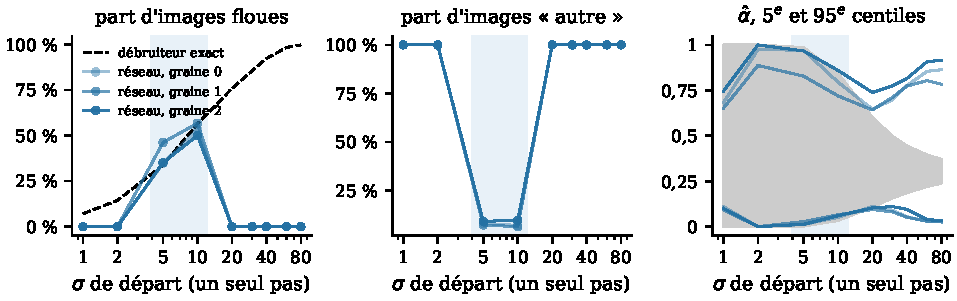
\includegraphics[width=\linewidth]{figures/fig_sigma.pdf}
  \caption{Diffusion échantillonnée en un seul pas depuis différents niveaux de bruit $\sigma$, pour les trois graines,
  comparée au débruiteur exact (en noir ou en gris). La bande bleue marque $\sigma = 5$ à 10, seule zone où le réseau suit la
  référence. À droite, la dispersion de la position $\ahat$ : celle de la référence se resserre autour de $p$ quand $\sigma$
  augmente, celle du réseau s'élargit.}
  \label{fig:sigma}
\end{figure}

Le réseau suit cette référence là où l'entraînement l'a beaucoup exposé, et seulement là. À $\sigma = 5$, il produit 35 à
46~\% d'images floues selon la graine, contre 34~\% pour le débruiteur exact ; à $\sigma = 10$, 50 à 57~\% contre 56~\%. La
dispersion de $\ahat$ y est comparable à celle de la référence, et moins de 10~\% des images sont classées \enquote{autre}. À partir de $\sigma = 20$, toutes ses images redeviennent \enquote{autre}, la distance médiane au
segment croît (de 0,21 à 0,23 selon la graine à $\sigma = 20$, de 0,36 à 0,41 à $\sigma = 80$), et la dispersion de $\ahat$ s'élargit (de 0,03 à 0,86 entre le 5\textsuperscript{e} et le
95\textsuperscript{e} centile à $\sigma = 80$) au lieu de se resserrer comme celle de la référence (0,24 à 0,37). Aux très
petits $\sigma$ (1 et 2), le réseau échoue aussi, mais pour une autre raison : le point de départ, un bruit pur de moyenne
nulle, s'écarte alors fortement des images bruitées vues à l'entraînement, dont la moyenne par pixel vaut $-0{,}77$.

Ce diagnostic est exploratoire et ne modifie pas la réponse à la question~2, rapportée telle que le critère la donnait. Il
indique cependant que l'échec à un pas tient à la couverture des niveaux de bruit pendant l'entraînement plutôt qu'à la
nature du problème.

\subsection{Q3 : les branches sont tirées dans la bonne proportion en moyenne, pas à chaque graine}

À 3 pas, la part de la branche A parmi les images nettes vaut 0,327, 0,255 et 0,358 selon la graine, pour $p = 0{,}3$
(figure~\ref{fig:calibration}, à gauche). La moyenne, 0,313, est proche de $p$, mais la troisième graine s'en écarte de
0,058, au-delà des 0,05 exigés pour chacune. Le critère fixé à l'avance demandait que les trois graines soient à moins de
0,05 de $p$ pour une réponse positive, et toutes au-delà pour une réponse négative : la question reste non tranchée. La
dispersion vient d'une graine à l'autre, pas de l'échantillonnage : chaque estimation repose sur plus de 1\,780 images
nettes, et ses intervalles de confiance à 95~\% sont larges d'environ $\pm 0{,}02$.

\begin{figure}[ht]
  \centering
  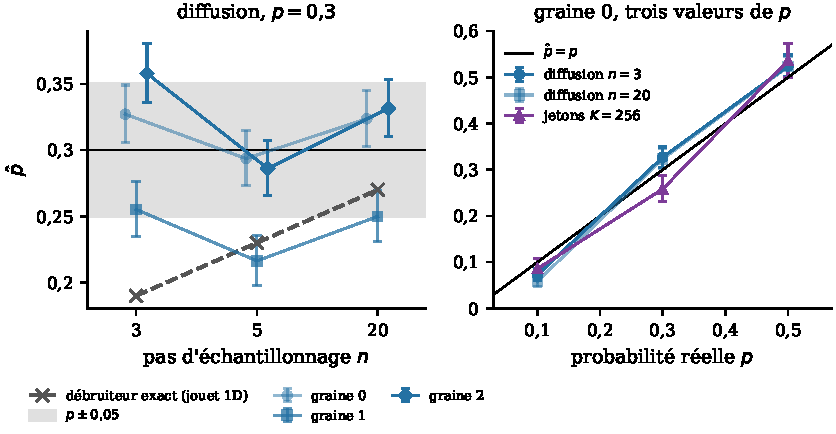
\includegraphics[width=\linewidth]{figures/fig_calibration.pdf}
  \caption{Proportion de la branche A parmi les images nettes, avec intervalles de confiance à 95~\%. À gauche, selon le
  nombre de pas de la diffusion, pour les trois graines ; la croix grise donne la prédiction d'un débruiteur exact en une
  dimension, échantillonné avec le même schéma d'Euler. À droite, selon la vraie probabilité $p$, pour une graine.}
  \label{fig:calibration}
\end{figure}

Deux observations nuancent ce résultat. D'abord, nous attendions un biais systématique plus fort. Un calcul préalable sur
un débruiteur exact en une dimension, échantillonné avec le même schéma d'Euler, prévoyait $\phat \approx 0{,}19$ à 3 pas,
par simple effet de la discrétisation. Le réseau entraîné est bien plus proche de $p$. Ensuite, la calibration n'est pas
monotone en $n$ : la moyenne sur trois graines vaut 0,313 à 3 pas, 0,265 à 5 pas et 0,302 à 20 pas.

L'axe $p$, mené sur une seule graine, ajoute une observation qui rejoint \textcite{um2024minority}. À $p = 0{,}5$, la diffusion
est calibrée (0,52 à 3, 5 et 20 pas). À $p = 0{,}1$, elle sous-représente la branche rare : $\phat = 0{,}072$ à 3 pas, 0,030
à 5 pas et 0,058 à 20 pas, avec des intervalles qui excluent tous 0,1 (figure~\ref{fig:calibration}, à droite). Les jetons,
eux, restent calibrés à $p = 0{,}1$ ($\phat = 0{,}086$). Une graine ne suffit pas à conclure, mais le sens de l'écart est celui
d'un débruiteur qui favorise la branche majoritaire.

\subsection{Q4 : le dictionnaire des jetons compte, mais pas pour le petit objet}

Le rappel du petit objet vaut 98,1~\% à $K = 64$ et 98,4~\% à $K = 1\,024$ (figure~\ref{fig:k}). L'écart, 0,2 point,
représente 0,76 écart-type poolé, loin des 3,23 requis : la question~4 reste non tranchée. Ce verdict ne signifie pas que $K$
est sans effet. Le rappel est en fait au plafond pour \emph{tous} les modèles de l'étude, entre 97,7 et 98,8~\%, y compris la
régression floue et l'oracle. Avec un objet de $2\times2$ pixels et un dictionnaire d'au moins 64 codes, la mesure retenue
ne pouvait pas départager les modèles.

\begin{figure}[ht]
  \centering
  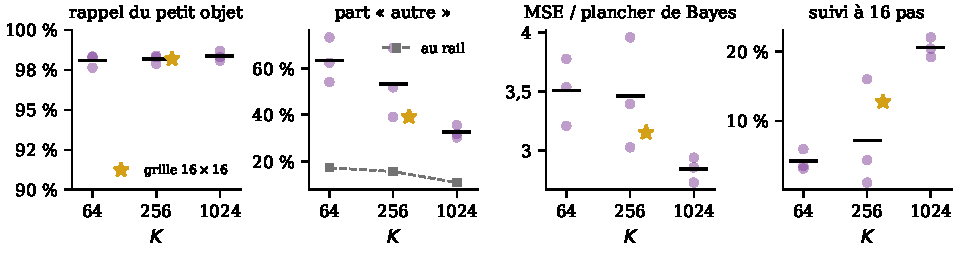
\includegraphics[width=\linewidth]{figures/fig_k.pdf}
  \caption{Modèles à jetons selon la taille $K$ du dictionnaire (points : graines ; trait : moyenne ; étoile : grille de
  $16\times16$ jetons à $K = 256$, une graine). Le rappel du petit objet ne bouge pas, les autres mesures s'améliorent avec
  $K$.}
  \label{fig:k}
\end{figure}

Les autres mesures, qui n'avaient pas de critère fixé à l'avance, évoluent toutes dans le même sens quand $K$ augmente. La
part d'images \enquote{autre} passe de 63~\% à $K = 64$ à 53~\% puis 33~\% à $K = 1\,024$ (de 17 à 11~\% sur le rail), l'erreur
de 3,51 à 2,84 fois le plancher, et le suivi à 16 pas de 4 à 21~\%. Un dictionnaire plus riche décrit mieux l'agent et
la scène, alors que la bifurcation elle-même est tranchée correctement quel que soit $K$. Affiner la grille à $16\times16$
jetons à $K = 256$ améliore aussi ces mesures (39~\% d'images \enquote{autre} contre 53~\%), pour un entraînement trois fois
plus long.

Le suivi à 16 pas éclaire aussi une question annexe : prédire la qualité d'un modèle sur 16 pas à partir de mesures sur un
seul pas. Sur les 9 modèles à jetons, la corrélation de rang avec le suivi à 16 pas vaut $-0{,}97$ pour l'erreur quadratique
par pixel et 0,59 pour le rappel du petit objet. Sur ce petit échantillon, l'erreur à un pas prédit mieux la qualité à long terme que le rappel.

\subsection{Q5 : le flou aide à estimer un risque immédiat, pas un risque lointain}

\paragraph{Mesure.} On retient les états de test où le risque de contact dans les $k$ pas suivants dépend de la branche, soit
265 états à $k = 1$, 419 à $k = 3$ et 552 à $k = 5$. Le coût exact $C^\star = p\,C_A + (1-p)\,C_B$ se calcule à partir des
deux futurs. Chaque modèle prédit les $k$ images suivantes en enchaînant ses propres prédictions, une fois pour la régression,
huit fois pour les générateurs, et l'on y lit le contact entre l'agent et l'ennemi. Le \emph{lecteur doux} mesure la part de
rouge sous la position de l'agent, une quantité affine en l'image ; le \emph{lecteur à seuil} répond oui ou non selon que
cette part dépasse 0,5. Avant toute mesure sur un modèle, nous avons vérifié que ce lecteur retrouve l'événement de contact
du jeu sur 100~\% de 30\,000 vraies images, dont 887 contacts.

\paragraph{Résultat.} La figure~\ref{fig:risque} donne l'erreur moyenne $\lvert \hat C - C^\star\rvert$. À un pas, les deux
critères fixés à l'avance donnent une réponse positive. Avec le lecteur à seuil, la régression se trompe de 0,30 en moyenne
contre 0,17 pour la diffusion à 3 pas, un écart de 0,14 et de 19,8 écarts-types poolés : son image floue ne franchit jamais
le seuil. Avec le lecteur doux, c'est l'inverse : la régression se trompe de 0,03 contre 0,16 pour la diffusion et 0,22 pour
les jetons. Le mélange contient la probabilité du contact, que le lecteur affine restitue directement, alors que les modèles
qui tranchent paient la variance de leurs 8 tirages. La diffusion fait à peine moins bien qu'un générateur parfait limité à
8 tirages (0,13), mesuré avec un prédicteur factice construit à partir du vrai jeu.

\begin{figure}[ht]
  \centering
  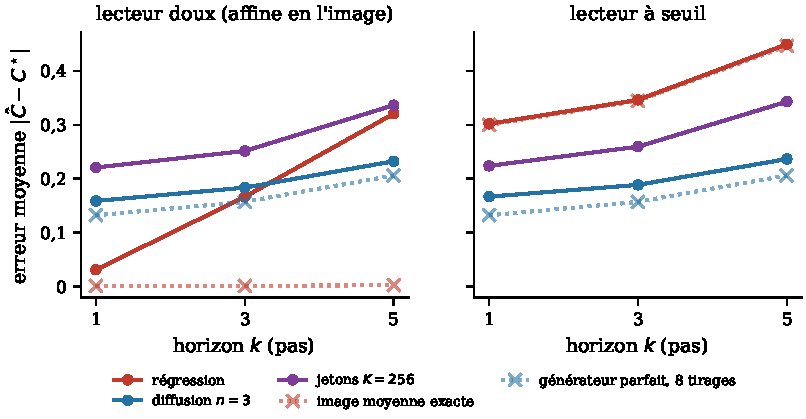
\includegraphics[width=\linewidth]{figures/fig_risque.pdf}
  \caption{Erreur d'estimation du risque de contact avec l'ennemi selon l'horizon $k$, moyenne sur trois graines. Les
  croix donnent deux références mesurées sans modèle entraîné : l'image moyenne exacte, et un générateur parfait limité à
  8 tirages.}
  \label{fig:risque}
\end{figure}

\paragraph{L'avantage disparaît avec l'horizon.} Au-delà d'un pas, l'erreur de la régression avec le lecteur doux croît
rapidement : 0,17 à $k = 3$ et 0,32 à $k = 5$, alors que l'image moyenne exacte resterait à 0,002. La diffusion passe de 0,16
à 0,23 seulement, et devient meilleure que la régression dès $k = 5$. La différence tient à ce que la régression reçoit en
entrée ses propres images floues, qu'elle n'a jamais vues à l'entraînement : c'est l'accumulation de biais contre laquelle
PETS met en garde \parencite[§5.2]{chua2018pets}. Ce résultat était exploratoire, sans critère fixé ; il nuance nettement la
lecture favorable au flou faite à un pas.

La figure~\ref{fig:rollouts} montre ce que voit un modèle quand il enchaîne ses prédictions. La régression floute l'ennemi à chaque
bifurcation (pas $t+1$, $t+7$ et $t+13$), puis reçoit ce mélange en entrée au pas suivant. La diffusion, elle, choisit une branche
et la suit de façon cohérente : ici, ce n'est pas celle qui s'est réalisée, mais c'est un futur possible. Pour les objets
déterministes, la régression reste la plus fidèle : l'agent et l'obstacle sont encore retrouvés à moins de 3 pixels après
16 pas dans 100~\% de ses trajectoires, contre 81~\% pour la diffusion à 3 pas et 7~\% pour les jetons à $K = 256$
(tableau~\ref{tab:principal}). C'est la représentation de l'événement aléatoire, et non la dynamique du reste de la
scène, qui dégrade l'estimation du risque de la régression aux horizons lointains.

\begin{figure}[ht]
  \centering
  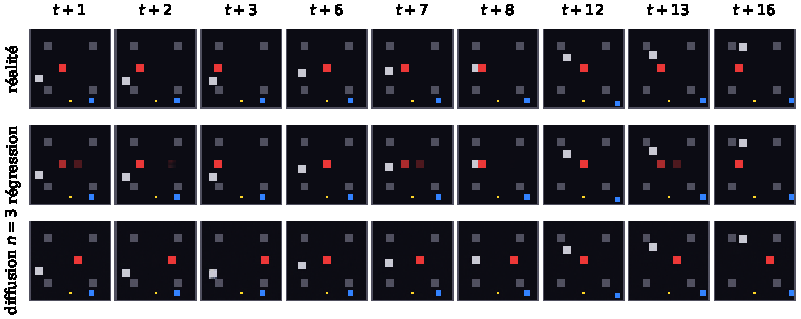
\includegraphics[width=\linewidth]{figures/fig_rollouts.pdf}
  \caption{Seize pas prédits à partir du même état de test, chaque modèle recevant ses propres prédictions en entrée (graine 0).
  En haut, ce qui s'est réellement passé. La régression dessine un ennemi double aux pas de bifurcation $t+1$, $t+7$ et $t+13$.
  La diffusion suit l'autre branche que celle de la réalité, de façon cohérente sur les seize pas.}
  \label{fig:rollouts}
\end{figure}

Nous n'avons pas mené la seconde partie prévue de cette étude, où un agent planifie ses actions dans le modèle à la manière
de PlaNet \parencite{hafner2019planet}. Son contrôle préalable est pourtant réussi : avec le vrai jeu comme modèle, le
planificateur subit 0,30 contact par partie et marque 4,9 points de plus que le bot aléatoire sur 20 parties. Le coût estimé,
de l'ordre de 15~heures de GPU pour un seul modèle à jetons, dépassait le budget disponible.

\subsection{Quand $p$ s'éloigne de 0,5, le classifieur ne voit plus le flou}

L'axe $p$ met en évidence une limite de l'instrument, connue dès sa conception mais qui devient visible ici
(figure~\ref{fig:p}). À $p = 0{,}1$, la régression est classée \enquote{nette} dans 98,6~\% des cas et floue dans aucun. Son
comportement n'a pourtant pas changé : son erreur vaut toujours 1,02 fois le plancher, et sa coordonnée moyenne
$\ahat = 0{,}095$ suit $p$. Le mélange $0{,}1\,A + 0{,}9\,B$ tombe simplement sous le seuil $\varepsilon = 0{,}2$, et
le classifieur le range parmi les images nettes-B. Une figure du flou en fonction de $p$ qui ne montrerait que la part
d'images floues suggérerait une conclusion fausse, à savoir que la régression cesse d'être floue quand l'événement devient
rare. Elle doit être lue avec $\ahat$ et le rapport au plancher.

\begin{figure}[ht]
  \centering
  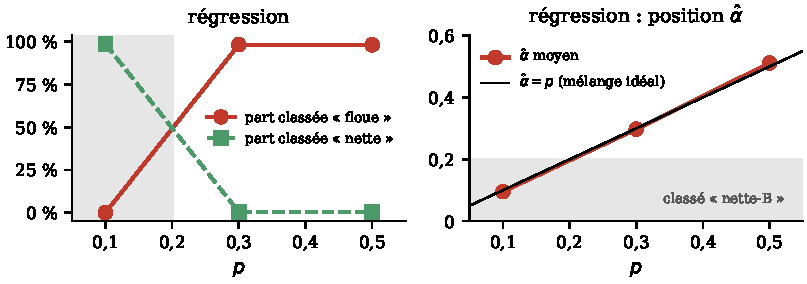
\includegraphics[width=0.85\linewidth]{figures/fig_p.pdf}
  \caption{Régression selon la probabilité $p$ (une graine). À gauche, la part d'images classées floues s'effondre à
  $p = 0{,}1$. À droite, la position moyenne $\ahat$ suit pourtant $p$ : le modèle produit toujours le mélange exact, mais
  celui-ci tombe dans la zone grisée que le classifieur range parmi les images nettes.}
  \label{fig:p}
\end{figure}

%% ============================================================================================================
\section{Discussion}\label{sec:discussion}

\paragraph{Le flou de la régression est une information, pas seulement un défaut.} La régression ne produit pas une image
approximativement floue : elle produit, à 1~\% près, l'espérance conditionnelle de l'image suivante. Cette image contient la
probabilité de chaque branche, et un lecteur affine peut l'exploiter mieux qu'un échantillon. C'est l'usage qui décide de la valeur du flou. Pour estimer un risque immédiat, il vaut mieux qu'un tirage ; pour simuler une trajectoire, il se dégrade
vite, parce que le modèle se retrouve face à des entrées qu'il n'a jamais rencontrées. Ce double constat rejoint celui de
\textcite{lambert2020objective} : la précision à un pas d'un modèle et son utilité pour le contrôle sont deux objectifs
distincts.

\paragraph{L'échec à un pas de la diffusion n'est pas celui de \emph{Boxing}.} DIAMOND observe qu'un pas unique moyenne les
futurs \parencite[§5.2]{alonso2024diamond}. Nous observons autre chose : un pas unique produit des images hors des futurs
possibles, y compris sur un jeu déterministe. Notre balayage du bruit de départ montre que le réseau se comporte comme le
débruiteur exact aux niveaux de bruit bien représentés à l'entraînement, et s'en écarte là où l'entraînement ne l'a presque
jamais exposé. Nous ne savons pas pourquoi DIAMOND n'observe pas le même échec ; une différence dans la distribution des
niveaux de bruit à l'entraînement, dans la taille du modèle ou dans les données est possible, mais nous ne l'avons pas
vérifiée. Notre résultat suggère surtout de regarder, avant d'interpréter un échantillonnage à très peu de pas, quels niveaux
de bruit l'entraînement a réellement couverts.

\paragraph{La calibration des modèles qui tranchent varie avec la graine.} En moyenne, la diffusion à 3 et 20 pas tire les
branches dans la bonne proportion, et mieux que ne le prévoyait le calcul sur un débruiteur exact. Mais d'une graine à l'autre,
la proportion varie de $\pm 0{,}05$ autour de $p$, et la branche rare semble sous-représentée à $p = 0{,}1$. Pour un modèle du
monde utilisé à estimer des fréquences d'événements, ces écarts ne sont pas négligeables : un événement de probabilité 0,1
prédit avec une fréquence de 0,03 à 0,07 serait sous-estimé d'un facteur 1,4 à 3,3.

\paragraph{Les jetons séparent deux sortes d'erreurs.} Les modèles à jetons tranchent la bifurcation aussi bien que la
diffusion, mais commettent davantage d'erreurs ailleurs dans l'image, surtout sur la position de l'agent. Ces erreurs
diminuent quand le dictionnaire grandit et s'accumulent sur 16 pas. Notre mesure du petit objet, elle, n'était pas assez
exigeante pour voir l'effet que nous cherchions.

%% ============================================================================================================
\section{Limites}\label{sec:limites}

\paragraph{Un seul jeu, très simple.} Toutes les conclusions portent sur un environnement de $64\times64$ pixels avec une seule
bifurcation à deux issues. Elles montrent ce que font ces familles de modèles quand l'incertitude est connue ; elles ne disent
pas comment ces comportements se combinent dans un jeu réel, où plusieurs événements aléatoires se superposent.

\paragraph{Peu de graines.} Les comparaisons principales reposent sur trois graines par famille, les axes $p$ et la grille fine
sur une seule. Avec trois graines, un effet de deux écarts-types a au mieux une chance sur deux d'être détecté (46~\% sans
correction pour les comparaisons multiples, moins avec). Les réponses non tranchées doivent donc se lire comme des absences
de preuve, pas comme des preuves d'absence.

\paragraph{Un budget égal en images, pas en calcul.} Les trois familles voient le même nombre d'images, mais un modèle à jetons
s'entraîne en environ une heure contre 2,5 pour les deux autres, et la taille des modèles varie de 12~\%. L'axe $K$ fait varier
à la fois le dictionnaire et le nombre de paramètres (de 5,91 à 6,59~M).

\paragraph{Les choix de l'instrument.} La part d'images \enquote{autre} dépend du seuil $\rho_{\max}$, réglé sur un bruit
synthétique, même si les conclusions résistent à un facteur 2 dans un sens comme dans l'autre. Le seuil $\varepsilon = 0{,}2$ empêche de voir le flou quand $p$ est proche de 0 ou de 1. La mesure restreinte au rail
réutilise un seuil calibré sur l'image entière. Enfin, aucune relecture humaine des classifications n'a été menée : la
correspondance entre les classes du classifieur et le jugement d'un observateur reste à établir.

\paragraph{Deux ajustements après le premier entraînement.} La taille du jeu d'entraînement (annexe~\ref{app:surapprentissage})
et celle du jeu de test, portée de 1\,000 à 2\,000 états pour que la question~3 puisse être tranchée, ont été modifiées après le
premier entraînement réel, avant toute comparaison entre familles. Ces deux changements s'appliquent identiquement à tous les
modèles, et le premier essai est conservé, mais ils rendent ces deux réglages moins indépendants des données que les autres.

%% ============================================================================================================
\section{Conclusion}\label{sec:conclusion}

Sur un jeu dont le hasard est entièrement connu, nous avons pu mesurer ce qui n'est habituellement que constaté. Une régression
à l'erreur quadratique dessine l'espérance exacte des futurs, à 1~\% de son minimum théorique. Un modèle de diffusion tranche
dès trois pas d'échantillonnage et tire les branches dans la bonne proportion en moyenne, avec une variabilité notable d'un
entraînement à l'autre. Un seul pas ne produit pas la moyenne attendue, et ce défaut se retrouve aux niveaux de bruit que
l'entraînement a peu couverts. Les modèles à jetons tranchent aussi, au prix d'erreurs sur le reste de l'image que la taille du
dictionnaire réduit.

Le résultat le plus utile pour l'usage des modèles du monde est peut-être le dernier. Le flou n'est pas un défaut absolu : il
porte la probabilité des issues, et un lecteur adapté en tire une meilleure estimation du risque immédiat qu'un échantillon.
Cet avantage disparaît dès que le modèle doit s'appuyer sur ses propres prédictions. Prolonger ce travail demanderait de
mesurer l'effet sur un agent qui planifie dans le modèle, la partie que notre budget n'a pas permis de mener, et de remplacer
le rappel du petit objet par une mesure capable de départager les modèles.

\printbibliography[heading=bibintoc, title={Références}]

%% ============================================================================================================
\newpage
\appendix

\section{Un premier essai écarté : la mémorisation des bifurcations}\label{app:surapprentissage}

Le premier entraînement réel, une régression à $p = 0{,}3$ sur 100\,000 transitions, a échoué au contrôle prévu pour cette
famille. Sur le jeu de test, son erreur valait 1,47 fois le plancher de Bayes, hors de l'intervalle $[1{,}00 ; 1{,}10]$, et
seulement 22,5~\% de ses images étaient classées floues, contre 97,6~\% après correction ; la proportion de la branche A parmi
ses images nettes valait 0,158.

Les courbes d'entraînement donnent la cause (figure~\ref{fig:surapprentissage}). Sur 34\,800 pas par lots de 64, le modèle voyait
chaque transition environ 22 fois. Sa perte de validation atteignait son minimum vers le pas 8\,000, puis remontait de 49~\%
jusqu'à la fin, pendant que sa perte d'entraînement continuait de baisser jusqu'à 0,46 fois le plancher de Bayes. Or ce
plancher ne peut être franchi qu'en connaissant la branche tirée : le réseau, qui ne la reçoit pas en entrée, avait appris par
c\oe ur l'issue de chacune des quelque 16\,700 bifurcations de son jeu d'entraînement. Il ne mesurait plus le flou inhérent
à l'erreur quadratique, mais sa capacité à mémoriser.

Porter le jeu d'entraînement à 400\,000 transitions (5,6 passages) supprime le phénomène : la validation reste stable (0,5~\%
au-dessus de son minimum en fin d'entraînement), la perte d'entraînement reste au-dessus du plancher, et le rapport au plancher
sur le test revient à 1,01. Le changement s'applique à toutes les familles et laisse le budget apparié intact. Le run
écarté n'entre dans aucune analyse ; ses journaux sont conservés dans le dépôt.

\begin{figure}[ht]
  \centering
  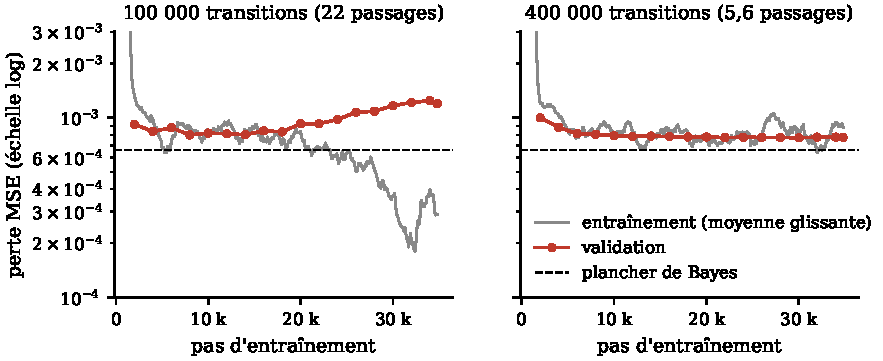
\includegraphics[width=\linewidth]{figures/fig_surapprentissage.pdf}
  \caption{Régression à $p = 0{,}3$ entraînée sur 100\,000 transitions (à gauche) et sur 400\,000 (à droite), avec le même
  nombre de pas. À gauche, la perte d'entraînement passe sous le plancher de Bayes et la validation remonte : le modèle
  mémorise l'issue des bifurcations. À droite, les deux courbes restent au-dessus du plancher.}
  \label{fig:surapprentissage}
\end{figure}

Cet incident a conduit à ajouter une alerte automatique aux courbes d'entraînement de chaque run. Elle se déclenche quand la
perte d'entraînement d'une régression passe sous le plancher de Bayes, ou quand la tendance de la perte de validation sur la
seconde moitié de l'entraînement est significativement croissante. Une première version, qui comparait le dernier point de
validation à son minimum, produisait de fausses alertes sur la diffusion, dont la validation fluctue fortement d'un relevé à
l'autre. Aucun des 25 entraînements retenus ne déclenche l'alerte corrigée.

\section{Critères fixés avant les calculs}\label{app:criteres}

\begin{table}[H]
  \centering\footnotesize
  \begin{tabularx}{\linewidth}{@{}lYYl@{}}
    \toprule
    Question & Réponse positive si & Réponse négative si & Résultat \\
    \midrule
    Contrôle de l'instrument & erreur moyenne sur $\ahat$ < 0,05 et plus de 99~\% d'images pures bien classées & sinon : aucune mesure de modèle & réussi \\
    Contrôle de la régression & rapport au plancher dans $[1{,}00 ; 1{,}10]$ à chaque graine, sans fuite & sinon & réussi \\
    Contrôles oracle et $p = 0$ & moins de 5~\% d'images floues & sinon & réussis \\
    \Q1 & flou de la régression > 50~\% et images nettes de la diffusion ($n = 3$) > 90~\% & flou de la régression < 30~\% ou flou de la diffusion > 10~\% & positive \\
    \Q2 & $n = 1$ plus flou que $n = 3$ d'au moins 10 points et de plus de 4,42 écarts-types (apparié) & écart < 10 points & négative \\
    \Q3 & $\lvert\phat - p\rvert$ < 0,05 à chaque graine (au moins 1\,000 images nettes) & $\lvert\phat - p\rvert \ge 0{,}05$ à chaque graine & non tranchée \\
    \Q4 & rappel à $K = 64$ inférieur à celui à $K = 1\,024$ de plus de 3,23 écarts-types poolés & écart de mauvais signe & non tranchée \\
    Contrôle du lecteur de contact & accord d'au moins 99~\% avec le jeu sur de vraies images & sinon & réussi \\
    Contrôle du planificateur & au plus 0,5 contact par partie et 3 points de plus que le bot aléatoire, avec le vrai jeu & sinon & réussi \\
    \Q5, lecteur à seuil & erreur de la régression supérieure à celle de la diffusion d'au moins 0,10 et de plus de 2,27 écarts-types & écart < 0,10 & positive \\
    \Q5, lecteur doux & erreur de la régression au plus égale à celle de la diffusion + 0,02 & supérieure de plus de 0,05 & positive \\
    \bottomrule
  \end{tabularx}
  \caption{Critères écrits avant les entraînements. Une réponse qui ne remplit aucune des deux conditions est non tranchée.
  Le seuil de 2,27 écarts-types de la question~5 n'est pas corrigé pour les comparaisons multiples : il appartient à une
  extension menée séparément des trois comparaisons principales. Les mesures dites exploratoires dans le texte (balayage du
  bruit, mesure restreinte au rail, effet de l'horizon, corrélations avec le suivi à 16 pas) n'avaient pas de critère.}
  \label{tab:criteres}
\end{table}

\section{Détails d'entraînement et d'échantillonnage}\label{app:details}

\paragraph{Commun aux trois familles.} Optimiseur AdamW ($\beta_1 = 0{,}9$, $\beta_2 = 0{,}99$, sans décroissance des poids),
taux d'apprentissage de $2\cdot10^{-4}$ atteint après 500 pas de montée linéaire puis décroissant jusqu'à 10~\% de cette
valeur, gradients écrêtés à une norme de 1, calcul en demi-précision. Entrée : les 4 dernières images empilées et l'action.
Validation tous les 2\,000 pas, point de reprise tous les 1\,000 pas.

\paragraph{Diffusion.} Préconditionnement d'EDM avec $\sigma_{\text{data}} = 0{,}5$, niveau de bruit d'entraînement
$\ln\sigma\sim\mathcal N(-1{,}2\,;\,1{,}2^2)$ \parencite{karras2022edm}. Échantillonneur d'Euler sur le calendrier de Karras,
avec $\sigma_{\max} = 80$, $\sigma_{\min} = 0{,}002$ et $\rho = 7$, pour $n \in \{1, 3, 5, 20\}$ pas. À $n = 1$, l'échantillon
est la sortie du débruiteur au niveau $\sigma_{\max}$.

\paragraph{Jetons.} Le VQ-VAE code chaque image en une grille de $8\times8$ jetons (ou $16\times16$ pour la grille fine) avec
une perte d'engagement \parencite{vandenoord2017vqvae} ; les codes inutilisés sont réinitialisés en cours d'entraînement. Il
reçoit 40~\% du budget, soit 13\,920 pas, et le Transformer causal les 20\,880 restants. Le Transformer prédit les jetons de
l'image suivante un par un, conditionné par les jetons du contexte et l'action, et l'échantillonnage se fait à température 1.

\paragraph{Mesure du risque.} Pour un état, le coût de contact à l'horizon $k$ est le nombre de pas, parmi les $k$ suivants, où
l'agent chevauche l'ennemi. Comme deux bifurcations sont séparées de 6 pas, une seule bifurcation intervient pour $k \le 5$, et
$C^\star = p\,C_A + (1-p)\,C_B$ est exact.

\section{Résultats par graine}\label{app:graines}

\begin{table}[H]
  \centering\footnotesize\setlength{\tabcolsep}{4pt}
  \begin{tabular}{@{}lcrrrrlr@{}}
\toprule
Modèle & graine & floue (\%) & nette (\%) & autre (\%) & images nettes & $\hat p$ [IC 95 \%] & MSE / plancher \\
\midrule
Régression & 0 & 98,2 & 0,4 & 1,4 & 8 & -- & 1,011 \\
Régression & 1 & 96,7 & 1,9 & 1,4 & 39 & -- & 1,016 \\
Régression & 2 & 97,9 & 0,7 & 1,5 & 13 & -- & 1,013 \\
\addlinespace
Diffusion, $n=3$ & 0 & 4,4 & 91,2 & 4,3 & 1825 & 0,327 [0,306 ; 0,349] & 2,044 \\
Diffusion, $n=3$ & 1 & 5,4 & 89,1 & 5,5 & 1783 & 0,255 [0,235 ; 0,276] & 1,896 \\
Diffusion, $n=3$ & 2 & 3,7 & 91,6 & 4,7 & 1833 & 0,358 [0,336 ; 0,380] & 2,115 \\
\addlinespace
Jetons, $K=256$ & 0 & 0,0 & 48,2 & 51,8 & 964 & 0,258 [0,231 ; 0,287] & 3,396 \\
Jetons, $K=256$ & 1 & 0,0 & 31,3 & 68,7 & 626 & 0,260 [0,226 ; 0,297] & 3,961 \\
Jetons, $K=256$ & 2 & 0,0 & 61,0 & 39,1 & 1219 & 0,313 [0,287 ; 0,340] & 3,025 \\
\bottomrule
\end{tabular}

  \caption{Mesures par graine pour le c\oe ur de l'étude ($p = 0{,}3$, 2\,000 états de test). L'intervalle de confiance de
  $\phat$ est l'intervalle binomial exact de Clopper-Pearson à 95~\%. Pour la régression, $\phat$ n'est pas donné, faute d'images nettes en nombre
  suffisant.}
  \label{tab:graines}
\end{table}

\section{Le débruiteur exact utilisé comme référence}\label{app:exact}

Notre jeu permet de calculer ce que ferait un débruiteur parfait, ce qui sert de référence au balayage du bruit
(figure~\ref{fig:sigma}) et à la question~3.

\paragraph{Forme fermée.} Pour un état donné, l'image suivante vaut $A$ avec la probabilité $p$ et $B$ sinon. Si l'on observe
$x = Y + \sigma\varepsilon$, avec $\varepsilon$ un bruit gaussien standard, le débruiteur qui minimise l'erreur quadratique
renvoie la moyenne a posteriori $D(x;\sigma) = w\,A + (1-w)\,B$, où $w$ est la probabilité a posteriori de la branche $A$ :
\begin{equation}
  \operatorname{logit} w \;=\; \operatorname{logit} p \;+\; \frac{\lVert x - B\rVert^2 - \lVert x - A\rVert^2}{2\sigma^2}
  \;=\; \operatorname{logit} p \;+\; \frac{\langle x,\, A - B\rangle}{\sigma^2} \;-\; \frac{\lVert A\rVert^2 - \lVert B\rVert^2}{2\sigma^2}.
\end{equation}
Un échantillonneur d'Euler à un pas part de $x = \sigma\,n$, un bruit pur, et renvoie $D(x;\sigma)$. Le terme
$\langle x, A-B\rangle/\sigma^2$ suit alors une loi normale centrée d'écart-type $\delta/\sigma$. Deux régimes en découlent. Si
$\sigma$ est grand devant $\delta$, ce terme est petit, $w$ reste proche de $p$ et l'image est le mélange flou attendu. Si $\sigma$
est petit devant $\delta$, le bruit tiré suffit à pousser $w$ vers 0 ou vers 1 : l'image sort nette, du côté choisi au hasard par
le bruit. Dans notre jeu, $\delta \approx 15{,}3$ en médiane à l'échelle du réseau. Les courbes de référence de la
figure~\ref{fig:sigma} sont obtenues sur les 2\,000 états de test, avec 40 tirages de bruit par état.

\paragraph{Pourquoi les très petits $\sigma$ ne sont pas interprétables.} Le réseau a été entraîné sur des images bruitées
$Y + \sigma\varepsilon$, dont la moyenne par pixel vaut celle des images du jeu, $-0{,}77$. Un bruit pur de niveau $\sigma$ a une
moyenne nulle, à $\sigma/\sqrt{12\,288}$ près pour une image de $64\times64\times3$ valeurs. Son écart à la moyenne attendue vaut
donc environ 85 de ces écarts-types à $\sigma = 1$, 8,5 à $\sigma = 10$ et 1,1 à $\sigma = 80$. Aux petits $\sigma$, le point de
départ est très loin de ce que le réseau a vu, et un échec y est attendu pour cette seule raison.

\paragraph{Le biais de discrétisation attendu.} La même forme fermée, réduite à une dimension, permet de simuler l'échantillonneur
d'Euler complet avec le débruiteur exact et le calendrier de bruit utilisé ($\sigma_{\max} = 80$, environ $5{,}3\,\delta$). Ce calcul
prévoyait $\phat \approx 0{,}19$ à 3 pas, 0,23 à 5 pas et 0,27 à 20 pas pour $p = 0{,}3$ : la discrétisation seule devait donc
sous-représenter la branche minoritaire. C'est la référence grise de la figure~\ref{fig:calibration}. Il s'agit d'une idéalisation
(une dimension, débruiteur exact), qui ne prédit pas le comportement du réseau entraîné : celui-ci s'est révélé bien plus proche de
$p$.

\section{Sensibilité au seuil $\rho_{\max}$}\label{app:sensibilite}

Le seuil $\rho_{\max}$ qui sépare les images \enquote{autre} des autres est réglé sur un bruit synthétique (section~\ref{sec:instrument}).
Le fichier d'évaluation de chaque modèle conserve $\ahat$ et $\rho$ pour chacun des 2\,000 états de test : on peut reclasser les mêmes prédictions avec un autre seuil, sans réévaluer les modèles (tableau~\ref{tab:sensibilite}).

\begin{table}[H]
  \centering\footnotesize
  \begin{tabular}{@{}lrrrrrr@{}}
\toprule
& \multicolumn{2}{c}{$\rho_{\max}\times0{,}5$} & \multicolumn{2}{c}{$\rho_{\max}$ (retenu)} & \multicolumn{2}{c}{$\rho_{\max}\times2$} \\
\cmidrule(lr){2-3}\cmidrule(lr){4-5}\cmidrule(lr){6-7}
Modèle & autre & floue & autre & floue & autre & floue \\
\midrule
Régression & 3,6 & 96,2 & 1,4 & 97,6 & 1,3 & 97,7 \\
Diffusion, $n=1$ & 100,0 & 0,0 & 100,0 & 0,0 & 100,0 & 0,0 \\
Diffusion, $n=3$ & 10,4 & 1,8 & 4,8 & 4,5 & 3,2 & 5,0 \\
Diffusion, $n=20$ & 3,6 & 0,0 & 3,5 & 0,0 & 3,3 & 0,0 \\
Jetons, $K=256$ & 54,1 & 0,0 & 53,2 & 0,0 & 52,5 & 0,0 \\
\bottomrule
\end{tabular}

  \caption{Part des prédictions classées \enquote{autre} et \enquote{floue} (\%) selon le seuil, moyenne sur trois graines à $p = 0{,}3$.
  Le seuil retenu vaut 0,160.}
  \label{tab:sensibilite}
\end{table}

Aucune conclusion du rapport ne change entre la moitié et le double du seuil. La diffusion à un pas reste à 100~\% d'images
\enquote{autre} même avec un seuil doublé : toutes ses images sont à plus de 0,32 du segment $[B, A]$, avec une distance médiane de 0,36 à 0,41 selon la graine. La
régression reste floue dans 96 à 98~\% des cas, et les jetons gardent 52 à 54~\% d'images \enquote{autre}. Seule la diffusion à
3 pas est sensible au seuil bas, qui fait passer une partie de ses rares images floues dans la catégorie \enquote{autre}.

\section{Reproduire ces résultats}\label{app:reproduire}

Le code et une copie légère des résultats de la campagne sont dans le dépôt du projet. Cette copie, d'environ 16~Mo, contient pour chacun des 25 entraînements ses mesures d'évaluation, son journal d'entraînement et les coordonnées $\ahat$ et $\rho$ de ses 2\,000 prédictions de test, mais pas les poids des réseaux. Toutes les figures et tous les tableaux de ce rapport s'en déduisent en quelques minutes, sans GPU, par un script unique (\texttt{rapport/make\_figures.py}). Les données d'entraînement se régénèrent à l'identique à partir de leurs graines, et les 25 entraînements se relancent par une seule commande, pour environ 47~heures sur un GPU T4.

\end{document}
